\documentclass[12pt]{article}

\usepackage{amssymb}
\usepackage{graphicx}
\usepackage{pgfplots}
\usepackage{rotating}
\usepackage{tikz}
\usepackage{xcolor}

\usetikzlibrary{shapes.geometric, arrows}
\graphicspath{ {./images/} }
\pgfplotsset{width=10cm, compat=1.9}

\tikzstyle{block} = [
    rectangle, rounded corners, minimum width=5cm, minimum height=0.8cm,
    text centered, draw=black
]
\tikzstyle{arrow} = [thick,->,>=stealth]

\begin{document}

\begin{titlepage}
    \begin{center}
        \vspace*{1.5in}

        \Huge
        Using the GPU to Accelerate Non-Destructive Image Editing

        \vspace*{2in}

        \Large

        Trinity Term 2022

        \vspace*{0.25in}
        Candidate Number: \emph{1034710}

        \vspace*{0.25in}
        Masters in Computer Science
    \end{center}
\end{titlepage}



\begin{center}
    \large \textbf{Abstract}
\end{center}

This project aims to a prove the concept for a general-purpose, non-destructive, GPU-accelerated
image editor.

For an image editor to be non-destructive, it must not destroy the source layers.  Therefore, it
must store every filter separately and recompute them whenever needed.  For the ideal user
experience, the user should be able to modify the `abstract' image (a tree of filters and layers)
and have an updated composite image appear on their screen within the next frame so the delay is
imperceptible.

Recomputing even parts of an image can be very computationally intensive, and, if we want to target
60 frames per second, then everything (including rendering the GUI) must happen with a latency of at
most 16.6ms.

To achieve such low latency and high throughput, I propose running \emph{all} the
image processing on the GPU---i.e. all the input textures are stored on the GPU, and the final
output is stored in a GPU texture that can then be drawn to the screen.  All the CPU does here is to
plan the sequence of commands for the GPU to execute; a task that is hard to implement but fast to
execute.

To determine if this is possible, I have implemented the `core' of an image editor using these
techniques.  I have then measured the latency of various image setups (TODO: add results).  To help
others building GPU-powered editors, I have also made accurate measurements of the latency and
throughput of various GPU operations.  (TODO: add results)

TODO: add conclusion, once I have results



\pagebreak

\tableofcontents



\pagebreak

\section{Introduction}

When image editing, the user's mental model of an edited image corresponds to a sequence of layers,
where each layer can be passed through any number of `filters', which are operations which modify
these layers (e.g. by moving, rotating, sharpening, adding blur, tweaking colours, etc.).  The
`filtered' version of the layers are finally merged (or `composited') together to form the final
`composite' image.

The ideal user experience for an image editor is one where the editor directly exposes precisely
this model and, when the user makes changes, instantly updates the composite image in the screen.
`Instant' means that the update latency is imperceptible, ideally within 16.6ms so that the new
image can be rendered in the same frame as the UI updates (assuming 60 frames per second).

Existing programs like Adobe Photoshop and Darktable shows us that fully non-destructive editing is
possible, but recomputing the image within a frame requires an enormous amount of computation.
Fortunately, almost all modern consumer computers contain extremely capable graphics processing
units (GPUs), which are designed to be extremely fast at highly parallel workloads such as image
processing.  Therefore, I propose running \emph{all} of the compute work on the same GPU that drives
the user's display.

This project aims to determine the feasibility of such a fully non-destructive, fully
GPU-accelerated image editor.  To do so, I have implemented a simple `core' of an image editor, and
used this to measure the latency of full GPU processing.  There are many further optimisations that
could be done, but they will not change the performance enough to change the feasibility result
(TODO: Update this once I actually have results).

TODO: Results



\pagebreak

\section{Background}

\subsection{Image Processing 101}

Image editors will largely be performing one of three types of operation:

\begin{enumerate}
    \item Per-pixel filters, where each pixel in the output is a simple function of either the same
        pixel in the input (e.g.\ brightness/contrast, hue/saturation/value) or the pixels near it
        (e.g.\ pick/hurl noise, edge detect/sharpen, small blurs).
    \item Transformations, where the image is translated, rotated or distorted in some way.
    \item Compositing, where a large number of `layers' are merged to form one final image.  See
        Figure~\ref{fig:compositing}.
\end{enumerate}

\begin{figure}
    \begin{center}
        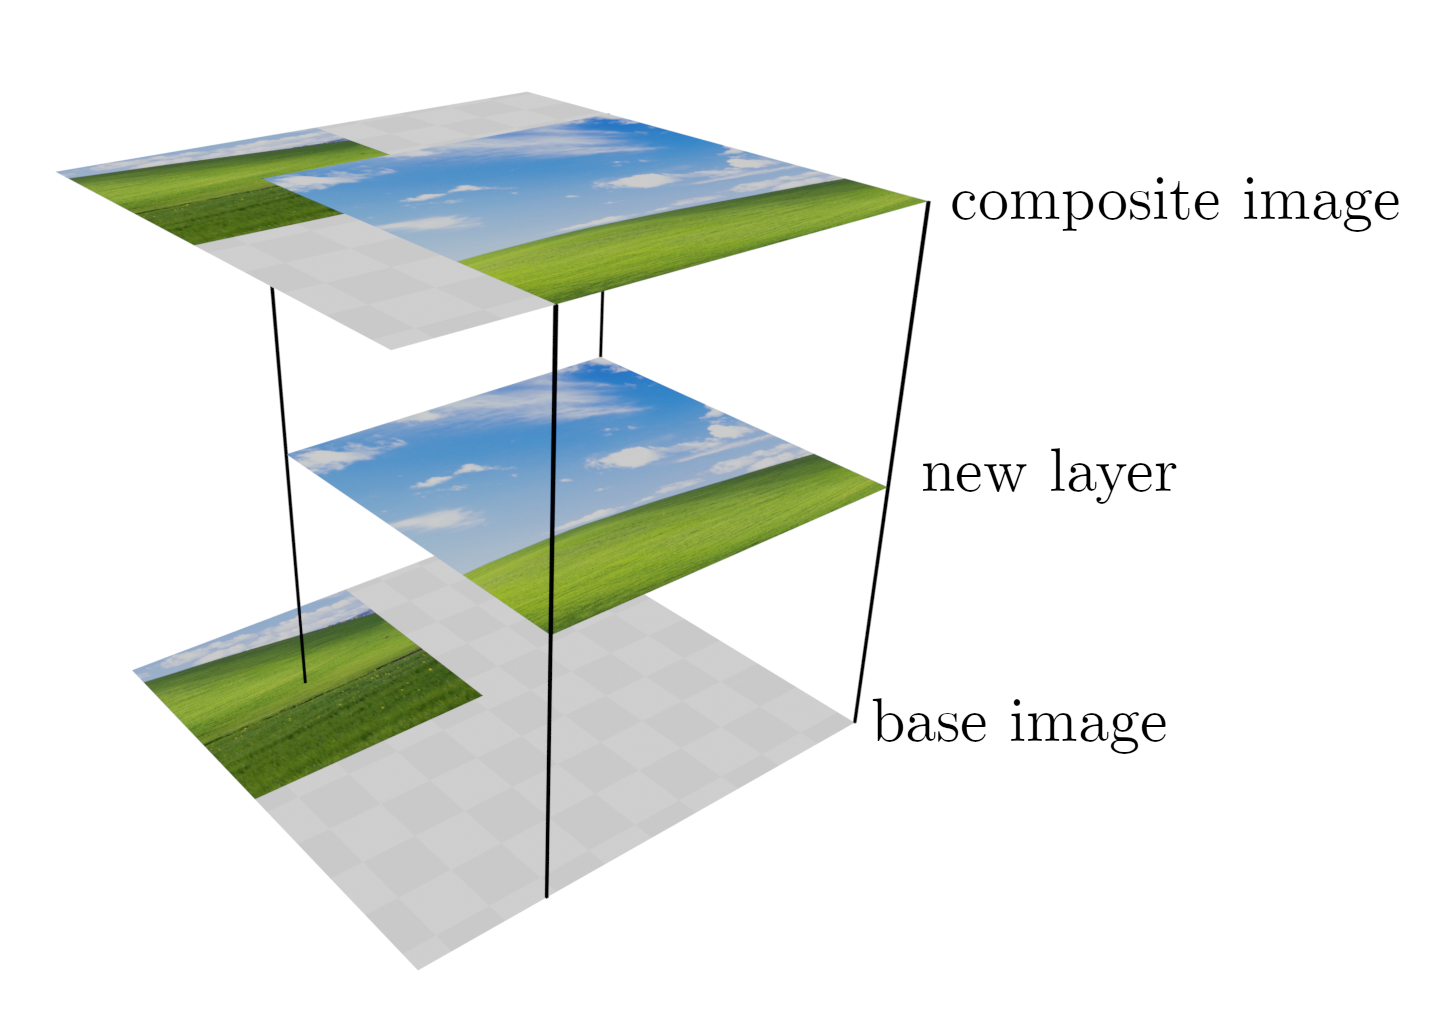
\includegraphics[width=0.6\textwidth]{compositing}
    \end{center}
    \caption{Compositing layers.  A base image is combined with a new layer (which only covers part
    of the image) to form a new image, with the new layer `above' the existing image.  Note how the
    top-left corner of the `new' image has overwritten the corner of the texture in base
    image.}\label{fig:compositing}
\end{figure}

All three of these are embarrassingly parallel---in each case, every pixel of the output can be
computed independently to all the others.

There are some image filters (like the various kinds of blur) which aren't as obviously
parallelisable, but there is still parallelisation opportunities (like computing 2D Gaussian blur by
combining horizontal and vertical blur passes, where each row/column is independent).



\subsection{Methods of Processing Images}

In a typical consumer computer, there are two main computation units which could be used for
processing images:

\subsubsection{The Central Processing Unit (CPU)}

Every computer contains a primary processor (the `Central Processing Unit' or CPU), which is
optimised for performing general computations on relatively small amounts of data.  There is some
parallelisation available, but CPUs are fundamentally optimised for fast sequential processing
rather than high parallelism.

Because of this, it's obvious that the CPU is a pretty inappropriate device for image processing.
The saving grace is that CPUs tend to have extremely high clock speeds and some degree of
parallelism: with multiple cores and SIMD, can perform upwards of 32 individual operations in
parallel at roughly 3GHz\footnote{According to Steam's Hardware Survey, CPUs have an average of 4.9
cores, as of April 2022, and almost all can perform 256-bit Single Instruction Multiple Data (SIMD)
instructions.  So, 32 parallel operations can be achieved if 4 cores are each performing operations
on eight 32-bit floating-point SIMD lanes in a 256-bit AVX register.  However, limitations like
memory speed and the sharing of functional units (thus causing logically different threads to
contest for the same hardware) make this theoretical limit very difficult to reach in practice.}.
This is fast enough that CPU-based processing is \emph{passable} but the latency and throughput are
both far from ideal.  Additionally, maxing out a computer's CPU tends to have a detrimental impact
on other threads running on the same machine---including other parts of the image editor, like the
GUI thread.

\subsubsection{The Graphics Processing Unit (GPU)}\label{sec:gpu}

Almost all modern computers also contain a secondary processor, the Graphics Processing Unit (GPU),
who's sole purpose is to accelerate graphics processing with a low latency and high throughput.

Some form of GPU is present in nearly every consumer device, with even low-powered mobile devices
featuring GPUs integrated into the same piece of silicon as the CPU.  Therefore, we can confidently
rely on graphics acceleration being present when writing consumer applications.  Note that this has
only recently been the case---over the last two decades, rising screen resolutions and refresh
rates made dedicated graphics processing go from exclusive to gaming to being ubiquitous in consumer
devices.

GPUs have two major processing modes:

\paragraph{Render passes:} Typically, a render pass involves taking 3D geometry, applying some
arbitrary transformation to the vertices, then performing some computation on every pixel of the
screen to compute its colour.  This is what GPUs are primarily designed for (it's what games need),
and is therefore GPUs have had many decades of optimisation relating to rendering efficiently.
Because rendering is a GPU's primary purpose, it means that render passes are available on any GPU.
Also, GPUs very often have custom hardware to make rendering as fast as possible.

To summarise, render passes are limited in the computation they can perform, but are extremely fast
and portable.  

\paragraph{Compute passes:} More recently, the raw power of GPUs has made people want to use them as
general purpose computing devices.  Any highly parallel tasks are very well suited to GPU
acceleration, including machine learning and (in our case) image processing.  Therefore, recent GPUs
can run arbitrary code on the same cores that would be used for rendering.  This has given rise to
General Purpose GPU (GPGPU) computing, which heavily utilises this ability.  Compute passes are
useful for doing operations that can't easily be represented as per-pixel operations, like
simulations or more complex filters such as Gaussian blur.

\subsection{Comparison of Compute APIs}

\subsubsection{CPU Compute (No API Needed)}

Computing images on the CPU is extremely simple, requiring no extra effort or clever APIs.  Source
images are loaded from disk into the CPU's memory as a flat array of pixel values.  Operations can
then be performed on those pixels using a plain \verb|for| loop.  Parallelisation can be achieved
using a combination of SIMD and multi-threading (splitting the pixels into chunks and having
different CPU cores process those chunks in parallel).  As described above, CPUs are easy to program
for but, on the whole, are ill-suited to the heavily parallel operations found in image processing.

\subsubsection{Graphics Libraries}

Controlling GPUs directly is an task, since you would be forced to deal with the differences between
every model of GPU.  To combat this, operating systems vendors (like Apple and Microsoft) or the
Khronos Group\footnote{https://www.khronos.org/} design APIs which provide users with a simpler
abstraction for the GPU, and require that GPU vendors implement this standard API in each GPU's
drivers.

The oldest and most well-known graphics API is OpenGL\footnote{https://www.opengl.org/}, first
released in in 1992 by the Khronos Group.  OpenGL is very high-level, which makes it easy to use for
simple cases (like making games) but lacks the low-level control required for achieving high
performance in more obscure cases (like image editors).

Armed with 24 years of hindsight, Khronos released Vulkan\footnote{https://www.vulkan.org/} in 2016
as a successor to OpenGL.  Meanwhile, Apple and Microsoft released
Metal\footnote{https://developer.apple.com/metal/} and
DirectX\footnote{https://en.wikipedia.org/wiki/DirectX}, respectively.  All of these modern APIs
favour a lower-level approach, requiring more code from their users but allowing much more
fine-grained control and potential for much better performance.

Until 2018, OpenGL and Vulkan where fully supported by all major operating systems (Windows, macOS,
Linux, iOS and Android).  In 2018, Apple announced that they would be deprecating OpenGL (along with
Vulkan and OpenCL) to encourage developers to use Metal.  As of 2022, OpenGL, Vulkan and OpenCL all
still work on Apple devices, but it is unclear for how long this will continue.  Code using Vulkan
can be used on Apple devices by using MoltenVK\footnote{https://github.com/KhronosGroup/MoltenVK} to
translate Vulkan function calls into Metal at runtime.  Similarly,
MoltenGL\footnote{https://moltengl.com/moltengl/} provides support for OpenGL, but both of these
only implement a subset of their corresponding APIs and are less than ideal.  The compatibility of
various APIs, along with OpenCL (discussed in Section~\ref{sec:open-cl}) and WebGPU (discussed in
Section~\ref{sec:wgpu}), is summarised in Figure~\ref{fig:apis-vs-oses}.

\begin{figure}
    \begin{center}
        \begin{tabular}{ c | c c c c c }
                    & Windows & macOS & Linux & iOS & Android \\
            \hline
            OpenCL  & \checkmark & deprecated   & \checkmark & deprecated   & \checkmark \\
            OpenGL  & \checkmark & subset       & \checkmark & subset       & \checkmark \\
            Vulkan  & \checkmark & subset       & \checkmark & subset       & \checkmark \\
            Metal   &            & \checkmark   &            & \checkmark \\
            DirectX & \checkmark \\
            \hline
            WebGPU & \checkmark & \checkmark & \checkmark & \checkmark & \checkmark
        \end{tabular}
    \end{center}
    \caption{Compatibility table of APIs against major operating systems.  iOS and Android are less
       relevant to image editors, but are included for completeness.}\label{fig:apis-vs-oses}
\end{figure}

\subsubsection{OpenCL}\label{sec:open-cl}

OpenCL\footnote{https://www.khronos.org/opencl/} (not to be confused with Open\textbf{G}L) is a
framework for running general compute operations on any hardware, also designed by the Khronos
Group.  OpenCL lets you write parallelisable C or C++ code once, then delegate that code to any
compute device (be that a CPU, GPU or anything else) at runtime.  Thus, the compute code only needs
to be written once.  This is a fantastic technology for high-throughput computation like machine
learning, but the increased throughput comes at the cost of increased latency (at least compared to
rendering geometry on a GPU).

As with OpenGL and Vulkan, OpenCL was fully portable until 2018, when Apple has also deprecated
OpenCL along with OpenGL and Vulkan.  Unlike the graphics APIs, no one has yet made a compatibility
layer like MoltenVK or MoltenGL (as far as I'm aware), so Apple devices still need to be handled as
a special case.  Finally, OpenCL, by its very nature as a \emph{compute} API, is required to use
\emph{compute} passes for its processing which, as described in Section~\ref{sec:gpu}, is not ideal
compared to render passes.

\subsubsection{WebGPU}\label{sec:wgpu}

WebGPU\footnote{https://www.w3.org/TR/webgpu/} is an in-progress standard to provide web
applications with low-level but safe access to general-purpose GPU acceleration.  WebGPU feels very
similar to Vulkan, and delegates to Vulkan, Metal or DirectX.  Therefore, WebGPU is extremely
portable, at the cost of not implementing some parts of Vulkan.  A Rust library,
\verb|wgpu|\footnote{https://github.com/gfx-rs/wgpu}, implements the WebGPU specification in a way
callable from native language like C, C++ and Rust.  \verb|wgpu| forms the core of Firefox's WebGPU
implementation, and is therefore very well-tested and stable.



\pagebreak

\section{State of the Art} % TODO: Should I call this 'Existing Editors'

\subsection{Adobe Photoshop}

I don't think Photoshop needs much of an introduction, since it has a near monopoly over image
editing---to the point where its name is synonymous with image editing itself.  To give an idea of
just how dominant Photoshop is, it has an estimated 26 million users
world-wide\footnote{https://prodesigntools.com/number-of-creative-cloud-subscribers.html}, including
90\% of the world's creative
professionals\footnote{https://www.adobe.com/about-adobe/fast-facts.html}.

\subsubsection{Non-Destructive Editing}

Since the introduction of Smart
Objects\footnote{https://helpx.adobe.com/photoshop/using/create-smart-objects.html} (and the
corresponding Smart Filters) in 2014, Photoshop has been able to implement most filters
non-destructively.  These are all computed on the CPU, though, so extensive use of Smart Filters
will often cause Photoshop to become noticeably slow.

\subsubsection{GPU Acceleration}

Photoshop runs almost all of its image processing on the CPU.  As of 2022, nine operations benefit
from GPU acceleration, whilst a further eight \emph{require} a
GPU\footnote{https://helpx.adobe.com/photoshop/kb/photoshop-cc-gpu-card-faq.html}.  It makes sense
that the Photoshop is not built with GPUs in mind---the first version of Photoshop was released in
1990\footnote{https://en.wikipedia.org/wiki/Adobe\_Photoshop}, nine years before the first consumer
GPU (Nvidia's GeForce 256) reached the market\footnote{https://en.wikipedia.org/wiki/GeForce\_256}.

Without access to Photoshop's source code, it's unclear exactly what APIs are being used this
GPU-acceleration.  Photoshop has settings for OpenCL, OpenGL, Vulkan and Metal, so I can only assume
that a combination of all four are used.  In summary, Photoshop appears to use largely CPU, with a
small amount of GPU compute passes and GPU rendering passes.

\subsection{GNU Image Manipulation Program (GIMP)}

The GNU Image Manipulation Program\footnote{https://gimp.org} (shortened to GIMP) is a free and open
source general-purpose image editor.  It has largely dominated the space of free image editing.

\subsubsection{Non-Destructive Editing}

As of 2022, all filters in GIMP are destructive, so there is no way to do non-destructive editing.
There is a plan to implement non-destructive
editing\footnote{https://www.gimp.org/docs/userfaq.html\#when-will-gimp-support-any-kind-of-non-destructive-editing-like-adjustment-layers-layer-filters-andor-full-blown-node-based-editing}
but that has not yet come to fruition.  It appears that GIMP's code is not written with
non-destructive editing in mind, and the addition appears to be a monumental refactoring task.

\subsubsection{GPU Acceleration}

GIMP has experimental support for GPU acceleration via OpenCL (first released in
2.10.0\footnote{https://www.gimp.org/news/2018/04/27/gimp-2-10-0-released/} in April 2018).  As of
2022, this is still experimental and is sometimes slower than CPU-based processing.  So, for most
users, GIMP is 100\% CPU-bound.

\subsection{Darktable}

Darktable\footnote{https://www.darktable.org/} is an open source `photography workflow application'
which features non-destructive editing which can be performed entirely on the GPU.  The only thing
really missing is that Darktable only supports a fixed pipeline of filters, rather than allowing the
user to choose how to compose them (this makes sense, because Darktable is only intended to be used
for adjusting photos).  Finally, Darktable uses OpenCL which, as described above in
Section~\ref{sec:open-cl}, is deprecated on Apple devices and can't take advantage of the
portability improvements from using render passes.



\pagebreak

\section{Implementation}

\subsection{Technologies Used}

The editing library is written in Rust, using \verb|wgpu| (see Section~\ref{sec:wgpu}) as the
graphics API\@.  \verb|wgpu| is an excellent library for this purpose---it provides low-level
control of the GPU in a way that is safe and runs on any major platform.  Not using native APIs
directly does create some overhead, but for a proof of concept the difference is negligible and the
portability and ease of use easily outweigh any small performance hit.  At any rate, there are many
better ways to optimise the prototype than using a different graphics library.

I also used WGSL (WebGPU's shading language) to write the shaders for the filters.  GLSL would
potentially have been easier, but the prototype doesn't need any complex shader logic and
\verb|wgpu|'s tutorials use WGSL so that's what I learned.

Finally, this report is written in \LaTeX\ and the 3D diagrams were made using a combination of
Blender\footnote{https://www.blender.org/} and GIMP.

\subsection{Notable Omissions}

This project is concerned with \emph{proving a concept} rather than with building a viable image
editor, so, as such, I have chosen not to implement many features that would be expected of a real
image editor but would not change the feasibility of a fully GPU-accelerated image editor.  Here, I
will quickly justify a few obvious omissions:

\subsubsection{Gaussian Blur and Other Blurs}

Running Gaussian blur efficiently on GPUs has been very thoroughly
researched\footnote{https://venturebeat.com/2017/07/13/an-investigation-of-fast-real-time-gpu-based-image-blur-algorithms/}
because of the applications in video games (for filters like bloom and depth of field) and GUIs and
the best algorithms, while slower than simple per-pixel filters, are very fast.  Approximation
techniques such as Kawase blur and Dual
blur\footnote{https://community.arm.com/cfs-file/\_\_key/communityserver-blogs-components-weblogfiles/00-00-00-20-66/siggraph2015\_2D00\_mmg\_2D00\_marius\_2D00\_notes.pdf}
give accurate results very quickly (though they are still approximations).  Other blur-like
operations (bloom, motion blur, glare, etc.) are also prevalent in video games and Kawase blur can
also be used to compute these efficiently.

\subsubsection{Brushes and Undo/Redo}

Brush systems and handling undo/redo are simply out of scope.  Implementing either in a GPU-friendly
way are, in their own right, worthy of projects but \emph{this} project is primarily concerned with
measuring the speed of processing image filters (processing brushes and undo/redo happen
occasionally, whereas image filters need to be processed many times per frame).  Handling brushes
and undo/redo are unlikely to have much impact on this because they both involve occasionally
modifying the source image textures.

Similarly, implementing a GUI is also out of scope.

\subsubsection{Caching}

Strategically caching the intermediate results of computations is a very effective way of reducing
the time required to update an image.  It is also particularly effective in practice, since when the
user makes lots of consecutive edits, they are almost always applied \emph{in the same place} of the
tree.  Thus, caching the intermediate layer just below this point will provide a large performance
boost.

For example, think about the user dragging a slider in a filter.  This will cause the image to
update nearly every frame, but all these updates will always change the same filter.  Therefore,
each frame the editor only has to recompute the filters on the path from the change to the root.

Whilst extremely effective, introducing caching makes the whole system substantially more complex.
It also doesn't make the performance any easier to evaluate---we are principally interested in
\emph{how much} image processing we can do within a frame.  Adding a caching system will only add
noise to these measurement.

\subsection{Design}

\subsubsection{Filter Types versus Filter Instances}

Before we explain the design of the prototype, it's worth emphasising the difference between a
filter \emph{type} and a filter \emph{instance}.

Intuitively, a filter \emph{type} is a generic version of a filter which is waiting for parameters,
whereas a concrete filter \emph{instance} supplies those parameters.  Therefore, `Gaussian blur',
`brightness/contrast' and `colour invert' are all filter \emph{types} (and are generic over some
parameters), whereas `Gaussian blur of radius 10 pixels' is a specific \emph{instance} of the
`Gaussian blur' \emph{type}.

Mathematically, a filter \emph{type} is a pair $(f, P)$ where $f: P \times \verb|image| \rightarrow
\verb|image|$ and $P$ is the set of possible parameters for the filter.  Each filter \emph{instance}
corresponds to a filter type $(f, P)$ and specific parameters $p \in P$.  Therefore, the result of
applying a filter \emph{instance} $((f, P), p)$ to an image $i$ is $f(p, i)$.

\subsubsection{Intermediate Textures versus Intermediate Layers}

In this project, there is a distinction between layers and textures: a texture is a concrete and
finite piece of data stored in the GPU's memory, while a layer is a conceptually infinite image.

Often, a layer will contain an image in some region and have transparency off to infinity in every
direction.  The unbounded nature of layers makes them impossible to compute directly, so instead we
store a finite \emph{region} of the layer in a texture.

\subsubsection{Lifetime of the Image Editor}

Before processing any images, the code must gain access to a GPU and initialise all the filter
types.  This involves mostly compiling the shader modules, but if filter types need any specific GPU
resources (like look-up textures) then those are also allocated here.

To initially load an image, all the referenced textures are read from disk, decompressed and copied
into GPU memory.  Once the textures are on the GPU, they can be freed from CPU memory.

Now, all the required resources are already on the GPU, so any updates to the image tree only
requires us to send the GPU a sequence of commands to recompute the new image.  The resulting
composite image ends up stored in a texture in GPU memory, ready to be rendered to the screen.
Determining a suitable sequence of GPU commands is where almost all of the complexity lies, so this
gets Section~\ref{sec:gpu-cmds} to itself.

If the image needs to saved to a file, then the composite image texture can be copied back into CPU
memory, encoded and finally written to disk as a file.  Otherwise, the final composite image is left
as a texture in GPU memory, ready to be rendered to the user's screen in the next frame.

This control flow is summarised in Figure~\ref{fig:control-flow}.  Note now all the expensive
operations, like compiling shaders and copying data between CPU/GPU memory, have been pushed out of
the `hot' code (updating the image, which could need to be run every frame) and into the `cold' code
(loading/saving images, which will happen quite rarely).

\begin{figure}
    \begin{center}
        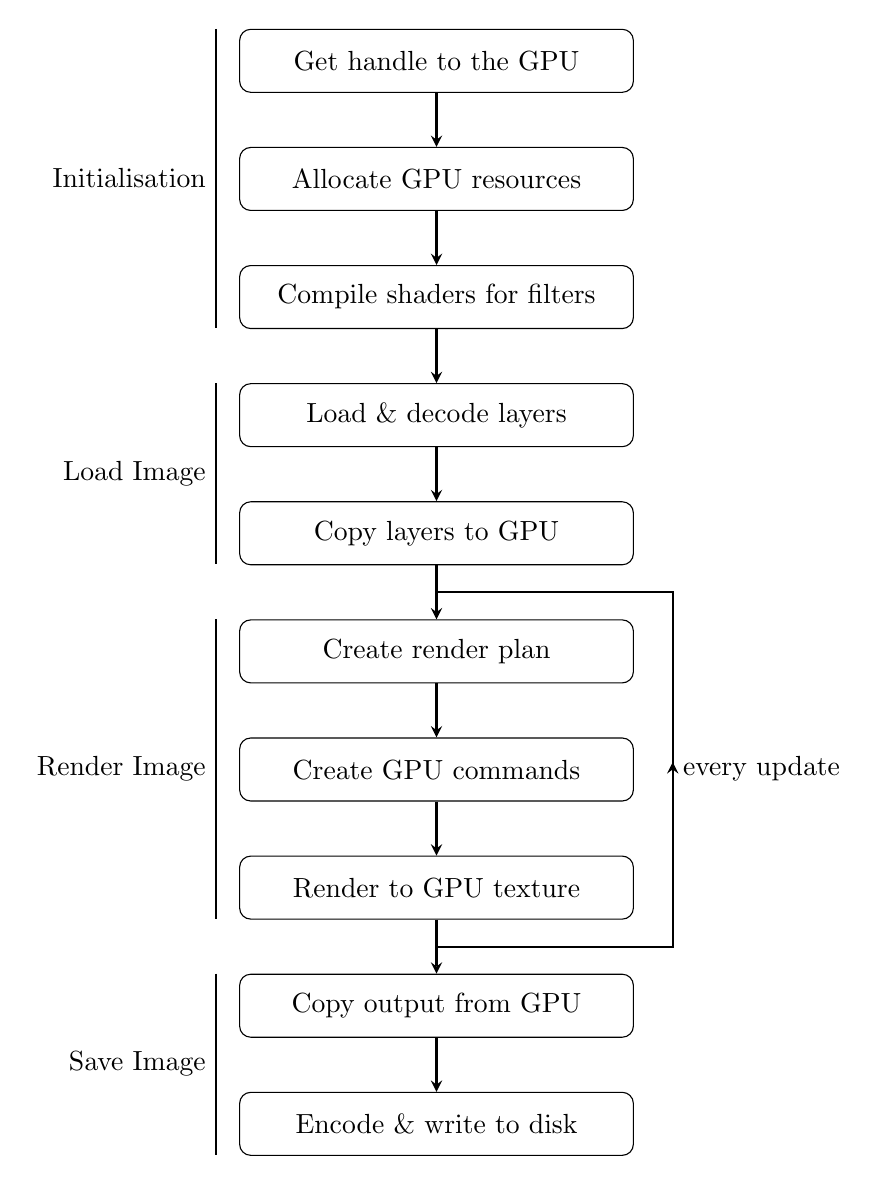
\begin{tikzpicture}[node distance=1.5cm]
            \node (init1) [block] {Get handle to the GPU};
            \node (init2) [block, below of=init1] {Allocate GPU resources};
            \node (init3) [block, below of=init2] {Compile shaders for filters};
            \draw [thick] (init1.north)+(-2.8,0) -- ++(-2.8,-3.8)
                            node[midway, anchor=east] {Initialisation};

            \node (load1) [block, below of=init3] {Load \& decode layers};
            \node (load2) [block, below of=load1] {Copy layers to GPU};
            \draw [thick] (load1.north)+(-2.8,0) -- ++(-2.8,-2.3)
                            node[midway, anchor=east] {Load Image};

            \node (render1) [block, below of=load2  ] {Create render plan};
            \node (render2) [block, below of=render1] {Create GPU commands};
            \node (render3) [block, below of=render2] {Render to GPU texture};
            \draw [thick] (render1.north)+(-2.8,0) -- ++(-2.8,-3.8)
                            node[midway, anchor=east] {Render Image};

            \node (save1) [block, below of=render3] {Copy output from GPU};
            \node (save2) [block, below of=save1] {Encode \& write to disk};
            \draw [thick] (save1.north)+(-2.8,0) -- ++(-2.8,-2.3)
                            node[midway, anchor=east] {Save Image};

            \draw [arrow] (init1) -- (init2);
            \draw [arrow] (init2) -- (init3);
            \draw [arrow] (init3) -- (load1);
            \draw [arrow] (load1) -- (load2);
            \draw [arrow] (load2) -- (render1);
            \draw [arrow] (render1) -- (render2);
            \draw [arrow] (render2) -- (render3);
            \draw [arrow] (render3) -- (save1);
            \draw [arrow] (save1) -- (save2);

            \draw [arrow] (render3.south)+(0,-0.35) -- +(3,-0.35) -- +(3,2);
            \draw [thick] (render1.north)+(0,0.35) -- +(3,0.35) -- +(3,-1.9)
                            node[anchor=west] {every update};
        \end{tikzpicture}
    \end{center}
    \caption{Control flow of the image editor.}\label{fig:control-flow}
\end{figure}

\subsubsection{Generating GPU commands}\label{sec:gpu-cmds}

To `compile' an image tree into a sequence of concrete GPU commands, this project takes heavily
inspiration from multi-pass compilers: we start with an `abstract' tree representing the image, then
`lower' this tree into a new tree with more annotations, then finally `lower' this intermediate tree
again into precise GPU commands\footnote{For those familiar with compilers, these correspond
(respectively) to the Abstract Syntax Tree (AST), an Intermediate Representation (IR) and the final
machine code.}.  Compared to its abstract counterpart (which is designed to be a nice interface for
the user of the library) this intermediate tree is both easier to optimise and easier to translate
into GPU commands.

In the case of this prototype, the `lowering' of the Abstract Tree to the Intermediate Tree is
simply a matter of labelling each filter and layer source with what GPU texture it should use, as
well as a bounding box of the region that we actually need (see Section~\ref{sec:virt-tex-spaces}
for more about these regions).

Finally, once we know what regions of which textures to use, generating the GPU commands becomes
fairly simple: every filter type exposes an function with signature like

\begin{verbatim}
trait FilterType {
    ...

    fn add_commands(
        &self,
        in: TextureRegion, out: TextureRegion,
        command_encoder: &mut wgpu::CommandEncoder,
    );
}
\end{verbatim}

For those not familiar with Rust, this declares a \verb|trait| containing a function with four
arguments: \verb|&self| is equivalent to the \verb|self| parameter in Python or \verb|this| in
object-oriented languages.  \verb|&self| is immutable, as opposed to \verb|&mut self| which would be
mutable.  \verb|in| and \verb|out| are two \verb|TextureRegion|s specifying the regions of virtual
and actual texture space on either side of the effect.  Finally, \verb|command_encoder| is a
\emph{mutable} reference to a \verb|wgpu::CommandEncoder|, to which the render/compute passes should
be added.

For per-pixel effects, this simply requires rendering a single quad that covers the correct region
of the output layer.  Getting the various coordinates (the quad's vertices and texture coordinates)
right is fiddly but not difficult.

\subsubsection{Virtual Texture Spaces}\label{sec:virt-tex-spaces}

When editing images, it is relatively common to encounter a situation where a layer is partially
outside the boundary of the whole image.  This presents an optimisation opportunity: sometimes we
only need to process filters for part of a layer, and if we can limit the size of the intermediate
textures, the processing will be faster because the GPU simply has to do less work.  In fact, there
are other ways that we can restrict the size of intermediate textures---any filter which throws away
information (masks, cropping, filling the layer with a solid colour, etc.) can also provide stricter
bounds for the filters below them.

Additionally, it would improve the consistency of the user experience if we are able to implement
transformation (translation, rotation, scaling, etc.) as \emph{just another filter}.  This allows
the user to intuitively create effects like stretching layers after blurring, as well as removing
layer positioning as a special case for the code to deal with.

It turns out that there's a simple way to achieve both of these: remove the requirement for the
origin of the intermediate textures to correspond to the origin of the larger layer they're trying
to represent.  I've dubbed these larger texture spaces `virtual', because the layer coordinates used
by the filters aren't anchored to any \emph{physical} texture.

This is illustrated in Figure~\ref{fig:virt-tex-space}.  See how the \verb|intermediate| textures
take up a rectangle in the middle of a larger texture space (in this case, the texture space of the
output image).  Also, see how the colour invert is only applied to the top-left region of
\verb|source_texture|, thus saving the GPU work.

\begin{figure}
    \begin{center}
        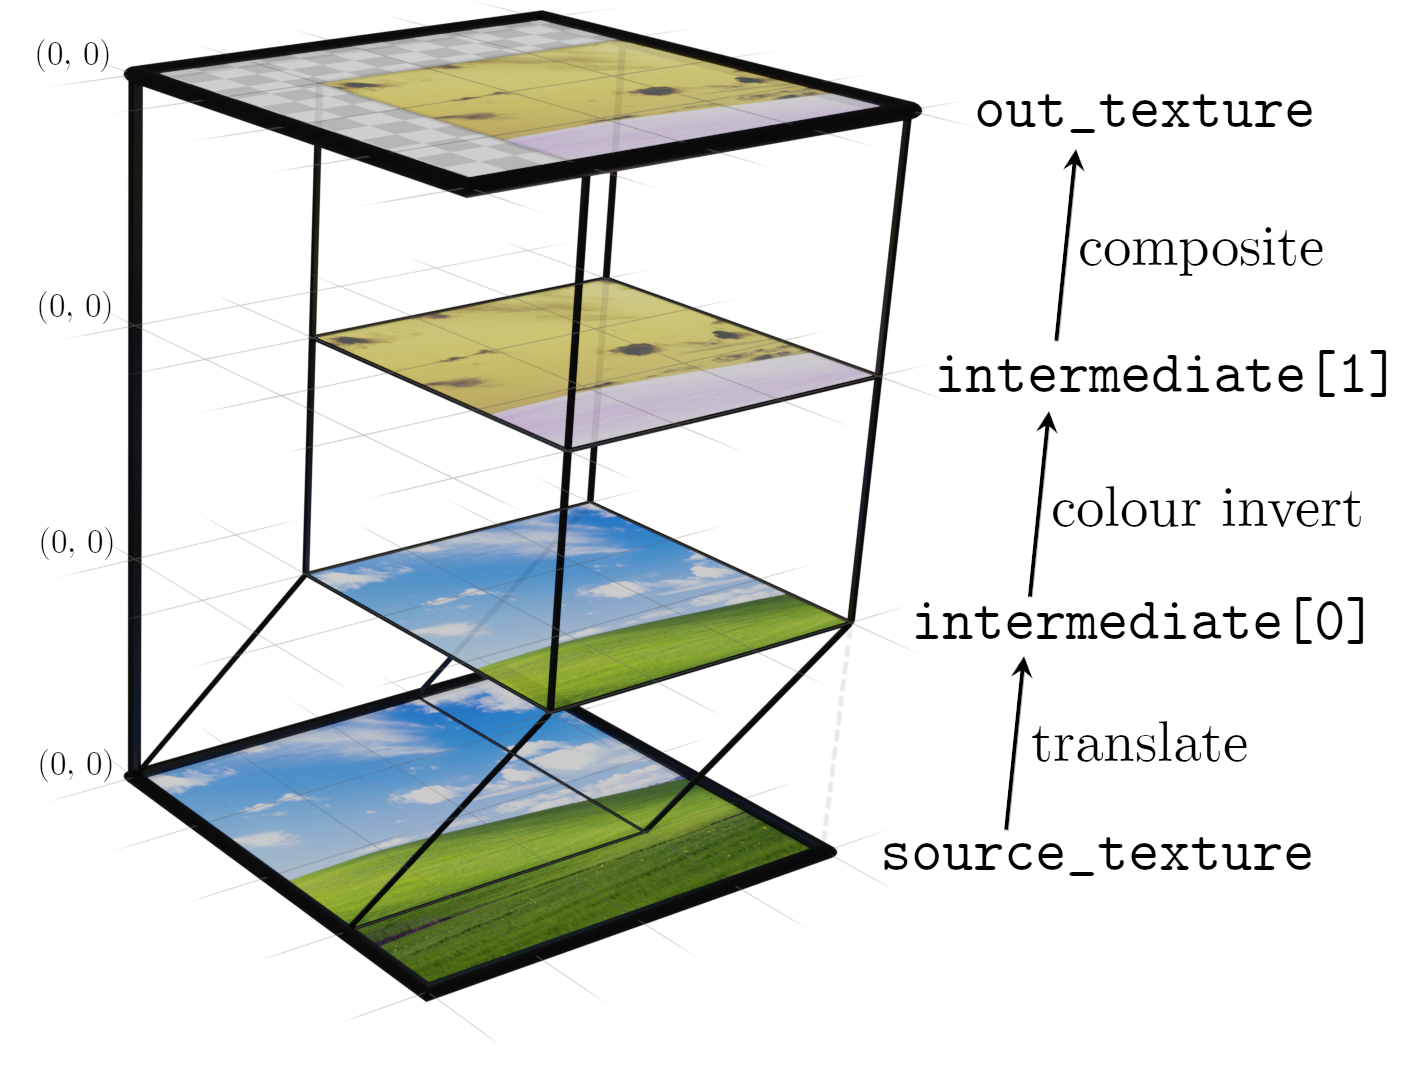
\includegraphics[width=0.9\textwidth]{filter-stacking}
    \end{center}
    \caption{Processing image filters using `virtual' texture space.  Note how the $(0, 0)$ points
    for both \texttt{intermediate} layers fall \emph{outside} the region stored in the
    texture.  Also note how the virtual texture spaces has allowed us to avoid processing nearly
    half of the source layer.}\label{fig:virt-tex-space}
\end{figure}

From the user's perspective, these virtual texture spaces are effectively infinite in every
direction.  By extension, this means that the user doesn't ever have to worry about layer
boundaries---the editor will automagically allocate enough texture space to fit the intermediate
layers.  If the user does somehow manage to create an enormous intermediate texture (e.g. by
scaling up by 1,000,000x, followed by scaling down by 1,000,000x), we can prevent disaster by
imposing a maximum intermediate texture size and only storing a very low-resolution version of the
oversized layer.  It's unlikely that the user would notice the difference, because the output
image is almost certainly smaller than this intermediate texture.  This means we have to compress
the data to get the output image, meaning that almost all of the extra information will be removed.
Anyway, I suspect that every other image editor would crash under such a situation; compared to
that, a bit of lost quality feels completely acceptable.

\subsubsection{Computing the Required Bounding Boxes}

The final piece of the puzzle is how we actually compute the bounding boxes for every layer.  We do
this in three passes: in the first, we start with the bounding box of the output image and propagate
this bounding box \emph{down} the chains of filters.  In the second pass, we start with the bounding box of
each source layer, and propagate this \emph{up} the chains of filters, until we reach output image
(which acts as the root of the image tree).  Finally, each layer is assigned the union of these two
bounding boxes (as in Figure~\ref{fig:bbox-compute}).  If we ever encounter an empty bounding box,
then everything below it cannot impact the output image and can just be removed from the
intermediate tree.

\begin{figure}
    \begin{center}
        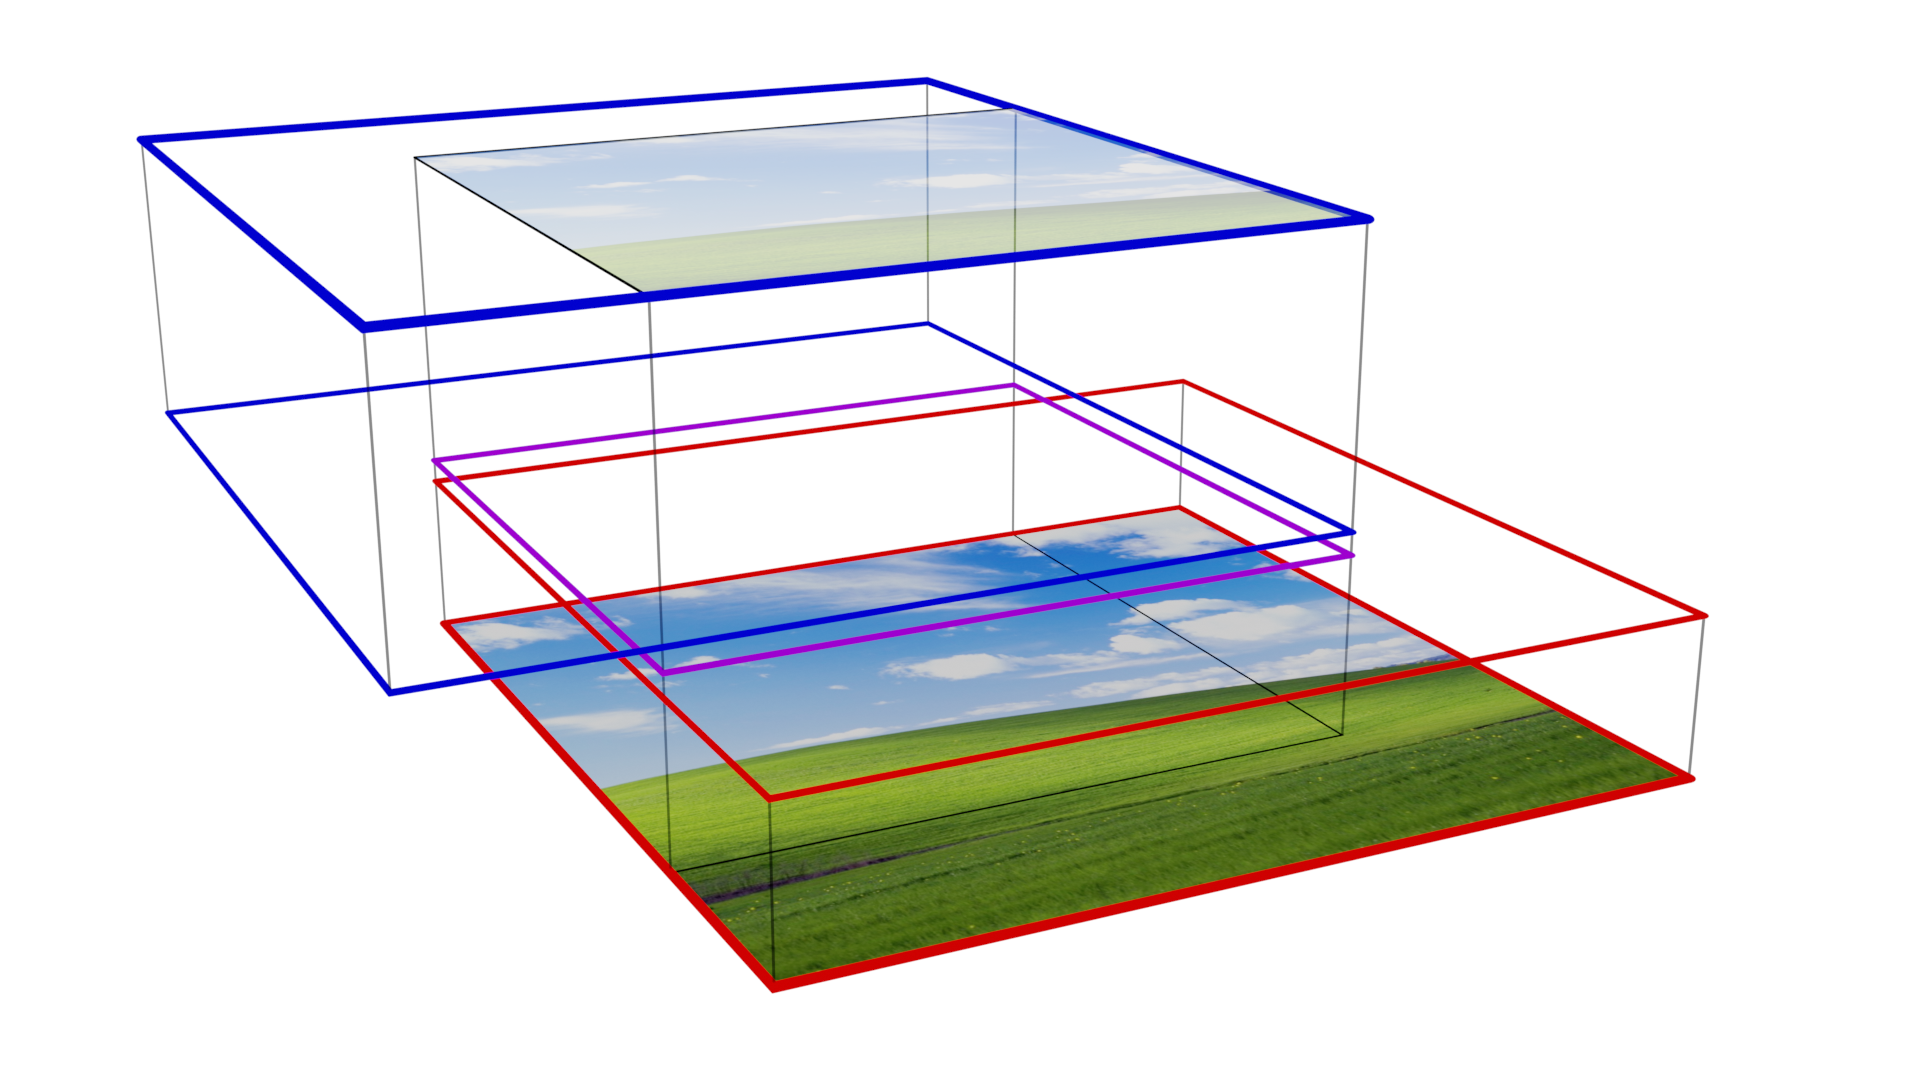
\includegraphics[width=0.9\textwidth]{bbox-compute}
    \end{center}
    \caption{Computing the bounding box for an intermediate layer.  In the first pass, the
    filter/layer above provides a bounding box (rendered in {\color{blue} blue}); in the second, the
    filter/layer below provides another bounding box (rendered in {\color{red} red}).  The region we
    have to compute (rendered in {\color{violet} purple}) is bounded by the union of these
    bounds.}\label{fig:bbox-compute}
\end{figure}

\subsection{Final Notes}

Conceptually, the design employed by this prototype is quite simple, but \verb|wgpu|'s verbose API
meant that the actual code ended up pretty large and complex.  In a real image editor, I strongly
recommend creating a hard abstraction boundary around the code that truly needs to control the GPU
and let the majority of the editor work at a higher level of abstraction.







\pagebreak

\section{Rogue Diagrams}

\begin{sidewaysfigure}
        \begin{verbatim}
Composite Image          Composite Image
 |                        |(out_texture)
 |- Layer #2              |- Layer #2               composite:
 |  |                     |  |(intermediate[0])       intermediate[0] -> out_texture
 |  |- Invert             |  |- Invert              render pass:
 |  |                     |  |(intermediate[1])       intermediate[1] -> intermediate[0]
 |  |- Transform          |  |- Transform           texture copy:
 |  |                     |  |(intermediate[0])       intermediate[0] -> intermediate[1]
 |  +- Source Image       |  +- Source Image        texture copy:
 |                        |    (source texture)       source_texture -> intermediate[0]
 +- Layer #1              +- Layer #1               composite:
    |                        |(intermediate[0])       intermediate[0] -> out_texture
    |- Contrast              |- Contrast            render pass:
    |                        |(intermediate[1])       intermediate[1] -> intermediate[0]
    +- Source Image          +- Source Image        texture copy:
                               (source texture)       source_texture -> intermediate[1]
                                                    clear: out_texture


   `Abstract' Tree          Intermediate Tree          GPU instructions
                        (annotated with textures)     (ordered bottom up)
        \end{verbatim}
    \caption{The `compiler' for GPU commands.  This is so hard to read that I don't think it's
    useful.}\label{fig:gpu-cmd-gen}
\end{sidewaysfigure}






\pagebreak

\section{Measurement Methodology}

\section{Results}


    \centering
    \begin{minipage}{0.5\textwidth}
        \centering
        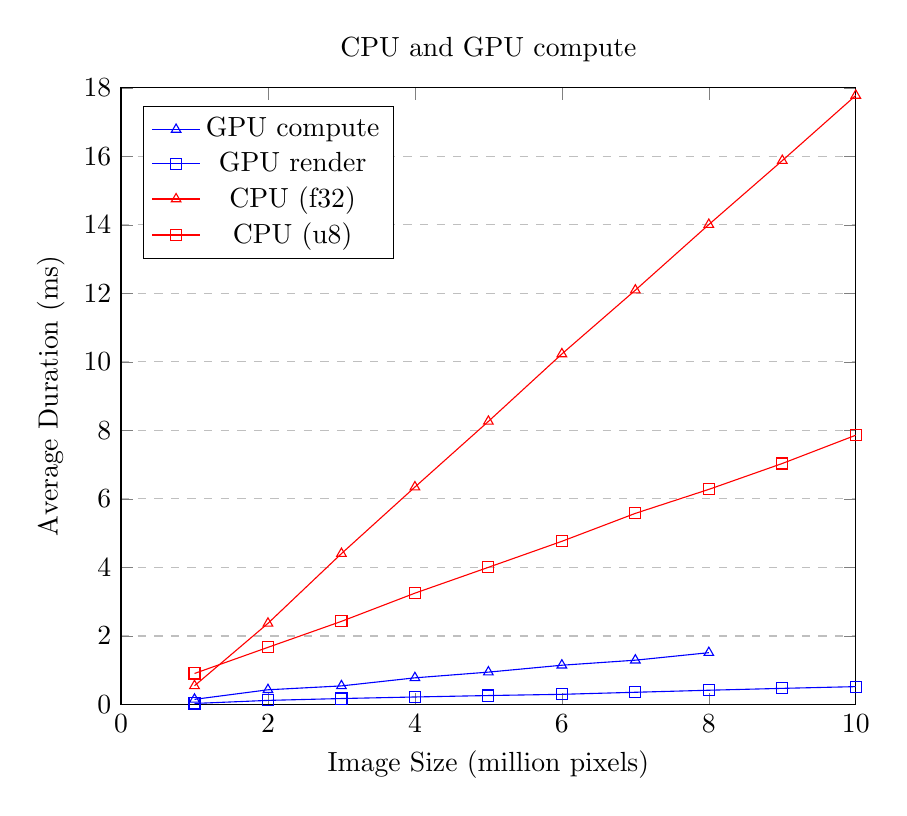
\begin{tikzpicture}
\begin{axis}[
    width=0.9\textwidth,
    title={ CPU and GPU compute },
    xlabel={ Image Size (million pixels) },
    ylabel={ Average Duration (ms) },
    xmin=0, xmax=10,
    ymin=0, ymax=18,
    xtick={ 0, 2, 4, 6, 8, 10 },
    ytick={ 0, 2, 4, 6, 8, 10, 12, 14, 16, 18 },
    legend pos=north west,
    ymajorgrids=true,
    grid style=dashed,
]
\addplot[color=blue, mark=triangle]
    coordinates { (1, 0.14930)(2, 0.42887)(3, 0.54195)(4, 0.77742)(5, 0.94439)(6, 1.14563)(7, 1.29275)(8, 1.51197) };
    \addlegendentry{ GPU compute }
\addplot[color=blue, mark=square]
    coordinates { (1, 0.02935)(2, 0.11899)(3, 0.17331)(4, 0.21855)(5, 0.26059)(6, 0.29627)(7, 0.35622)(8, 0.41557)(9, 0.47030)(10, 0.52086) };
    \addlegendentry{ GPU render }
\addplot[color=red, mark=triangle]
    coordinates { (1, 0.54529)(2, 2.36894)(3, 4.40375)(4, 6.34718)(5, 8.26329)(6, 10.23192)(7, 12.09424)(8, 14.00943)(9, 15.87651)(10, 17.77921) };
    \addlegendentry{ CPU (f32) }
\addplot[color=red, mark=square]
    coordinates { (1, 0.90488)(2, 1.66785)(3, 2.42644)(4, 3.24934)(5, 4.00376)(6, 4.76293)(7, 5.57851)(8, 6.27884)(9, 7.03501)(10, 7.86027) };
    \addlegendentry{ CPU (u8) }

\end{axis}
\end{tikzpicture}
    \end{minipage}\hfill
    \begin{minipage}{0.5\textwidth}
        \centering
        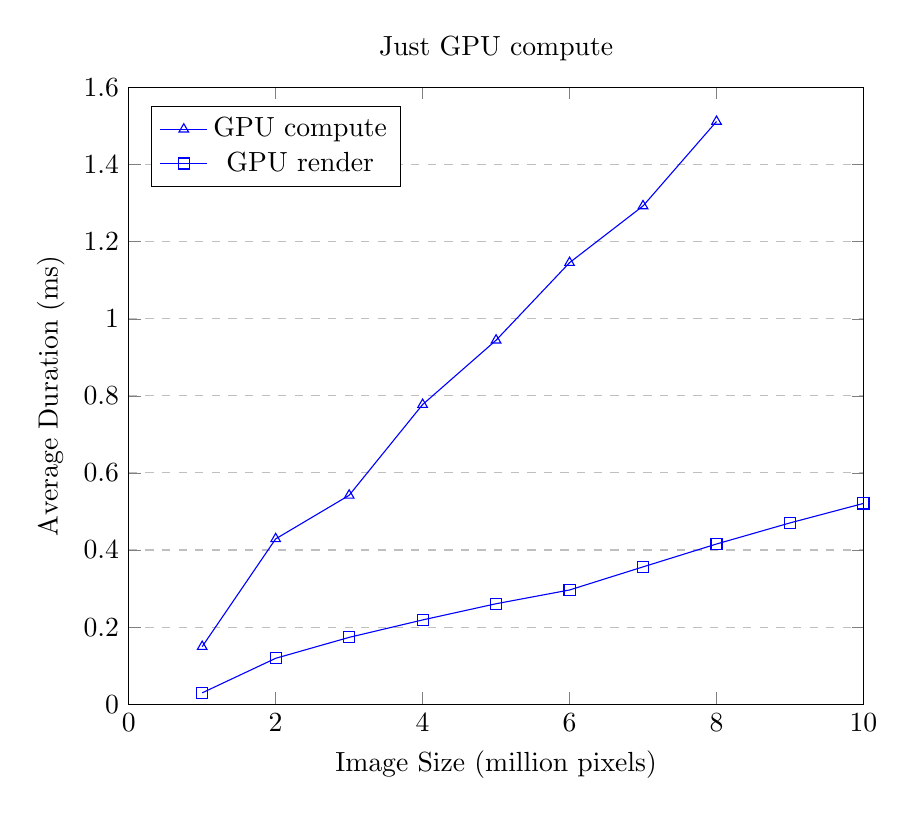
\begin{tikzpicture}
\begin{axis}[
    width=0.9\textwidth,
    title={ Just GPU compute },
    xlabel={ Image Size (million pixels) },
    ylabel={ Average Duration (ms) },
    xmin=0, xmax=10,
    ymin=0, ymax=1.6,
    xtick={ 0, 2, 4, 6, 8, 10 },
    ytick={ 0, 0.2, 0.4, 0.6000000000000001, 0.8, 1, 1.2, 1.4, 1.5999999999999999 },
    legend pos=north west,
    ymajorgrids=true,
    grid style=dashed,
]
\addplot[color=blue, mark=triangle]
    coordinates { (1, 0.14930)(2, 0.42887)(3, 0.54195)(4, 0.77742)(5, 0.94439)(6, 1.14563)(7, 1.29275)(8, 1.51197) };
    \addlegendentry{ GPU compute }
\addplot[color=blue, mark=square]
    coordinates { (1, 0.02935)(2, 0.11899)(3, 0.17331)(4, 0.21855)(5, 0.26059)(6, 0.29627)(7, 0.35622)(8, 0.41557)(9, 0.47030)(10, 0.52086) };
    \addlegendentry{ GPU render }

\end{axis}
\end{tikzpicture}
    \end{minipage}
    

\section{Conclusion}



\pagebreak

\begin{thebibliography}{99}
\end{thebibliography}

\end{document}
